\chapter{Computational Results for Mean-Variance Setup}

We analyze the performance of robust portfolio optimization methods discussed in the preceding chapter vis-\`a-vis the Markowitz model in a practical setup involving domestic market data and simulated data. The analysis is performed under two scenarios, namely, the number of stocks \textit{N} being 31 and the number of stocks \textit{N} being 98. This is done in order to observe the effect of increase in number of stocks on the performance of robust methods with respect to the Markowitz model. These numbers were chosen since they represent the number of stocks in S\&P BSE 30 and S\&P BSE 100 indices, respectively.

For the first scenario, we use the daily log-returns based on daily adjusted close price of the 31 stocks comprising BSE 30 (data source: Yahoo Finance \cite{yf}). Accordingly, we have considered the period from December 18, 2017 to September 30, 2018 (both inclusive) comprising of a total of 194 active trading days. Corresponding to this market data, we prepare two sets of simulated data for the 31 assets by sampling returns from a multivariate normal distribution with mean and covariance matrix set equal to those obtained from the S\&P BSE 30 data. The first set of sample returns comprises of number of samples same as the daily log-return observations in S\&P BSE 30 market data, namely, 193, whereas the second set comprises of 1000 samples. The two sets of simulated sample returns of different sizes were used to facilitate the study of the impact of the number of samples in simulated data on the performance of the robust portfolio optimization approaches. We make a comparative study of robust portfolio optimization approaches, in case of the historical S\&P BSE 30 data, as well as the two sets of simulated data, in order to analyze whether the worst case robust portfolio optimization approaches are useful in a real market setup.

For the second scenario, we use the log-returns based on daily adjusted close price data of the 98 stocks comprising S\&P BSE 100 (data source: Yahoo Finance \cite{yf}) with the period spanning from December 18, 2016 to September 30, 2018. Two sets of simulated data are constructed using multivariate normal distribution, on the similar lines as the first scenario. Similar kind of comparative study is performed for the second scenario.

The robust portfolio optimization approaches that we have taken into consideration for analyzing their performance with respect to Markowitz model without short-selling (\textbf{Mark}) are as follows:
\begin{enumerate}
    \item{Robust Model involving box uncertainty set in expected return without short-selling (\textbf{Box}).}
    \item{Robust Model involving ellipsoidal uncertainty set in expected return without short-selling (\textbf{Ellip}).}
    \item{Robust Model involving separable uncertainty set without short-selling (\textbf{Sep}).}
\end{enumerate}
For Box and Ellip model, we construct uncertainty sets in expected mean return with $100(1-\alpha)\%$ confidence level by considering $\alpha=0.05$. Separable uncertainty set in Sep model is constructed as a $100(1-\alpha)\%$ confidence interval for both $\mu$ and $\Sigma$ using Non-parametric Boostrap Algorithm with same $\alpha$ as in other robust models and assuming $\beta$, \textit{i.e} the number of simulations, equal to 8000.

The performance analysis for these robust portfolio models vis-\`a-vis the Mark model is performed by taking into consideration the \say{Sharpe Ratio} of the portfolios constructed having $\lambda$ representing risk-aversion in the ideal range \cite{fabozzi} \textit{i.e.}, $\lambda \in [2,4]$. Since the yield for Treasury Bill in India from 2016 to 2018 has been found to oscillating around $6\%$ \cite{rbi}, so, we have assumed the annualized riskfree rate to be equal to $6\%$. In the following sections, we present the computational results observed in case of two scenarios as discussed above.

\section{Performance with $N=31$ Assets}

We begin with the analysis for $N=31$ assets, in the case of the simulated data with $1000$ samples. In Figure \ref{fig:1} and Table \ref{tab:1}, we present the efficient frontier and performance of portfolios constructed by applying the Mark model and three robust models to the simulated returns. We observe that efficient frontiers for the Ellip and Sep models lie below the one for the Mark model. This supports the argument made by Broadie \cite{Broadie} regarding over-estimation of efficient frontier in case of the Mark model. Overlap of efficient frontiers for the Mark and Box models indicates that utilizing box uncertainty set for robust optimization does not prove to be of much use in this case. This claim is supported quantitatively from Table \ref{tab:1} as well as since the average Sharpe ratio for portfolios constructed in the ideal range of risk-aversion is same in case of both the models. From Table \ref{tab:1}, we infer that Sep model performs at par with Mark model if we take into consideration the average Sharpe Ratio. This is evident from Figure \ref{fig:1} as well, since Mark model starts outperforming Sep model in terms of Sharpe ratio after the risk-aversion crosses 3. We also note that the Ellip model outperforms all the models including the Mark model in the entire ideal range of risk-aversion.


\begin{figure}[!h]
    %\centering
    %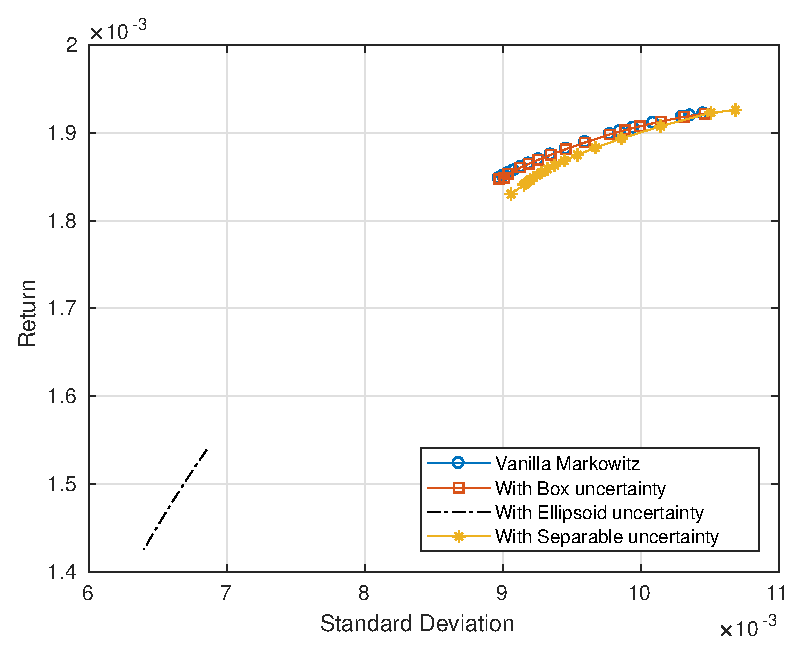
\includegraphics{bse30_simulated/ef_ideal_range_1000_sim.eps}
    %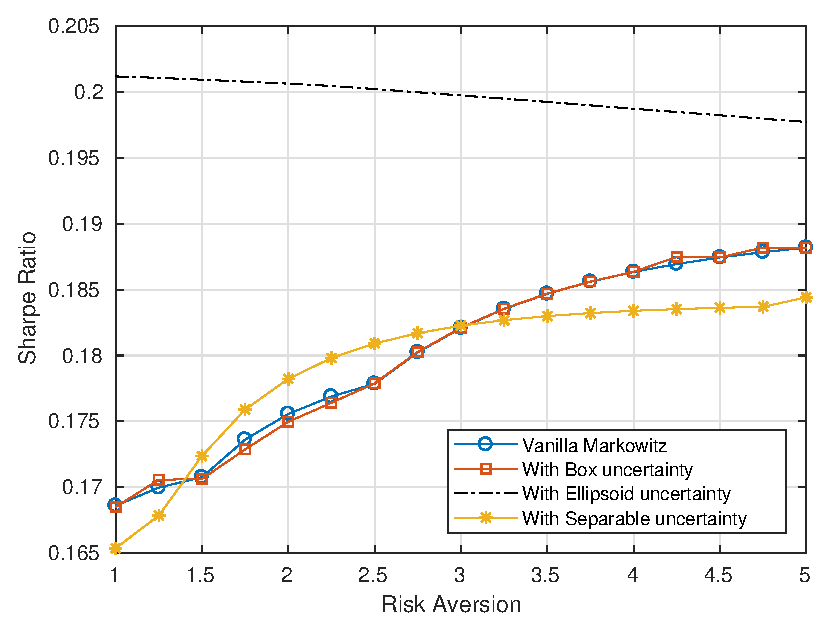
\includegraphics{bse30_simulated/sr_ideal_range_1000_sim.eps}
    
    %\label{fig:1}
    \subfloat{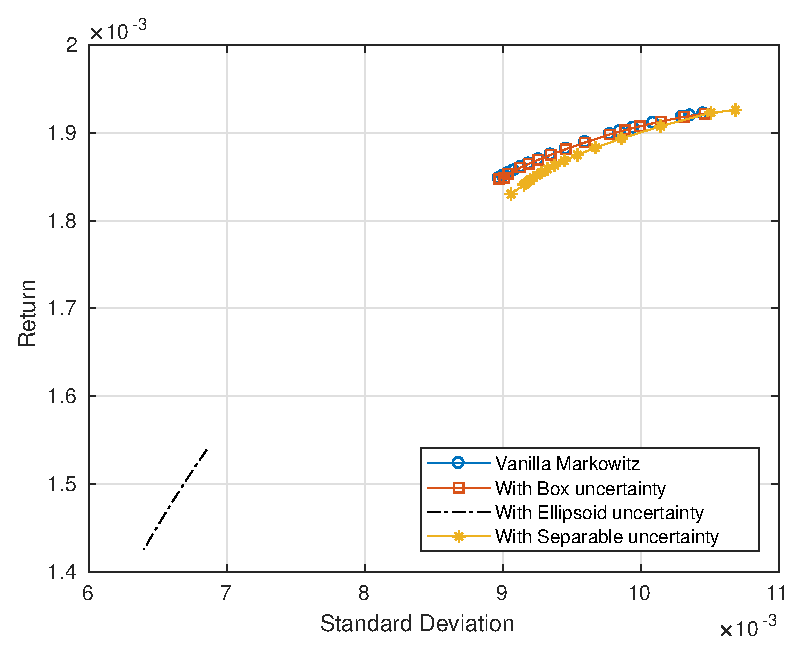
\includegraphics[height=6.9cm,width=0.5\textwidth]{bse30_simulated/ef_ideal_range_1000_sim.eps}} \hfill
   \subfloat{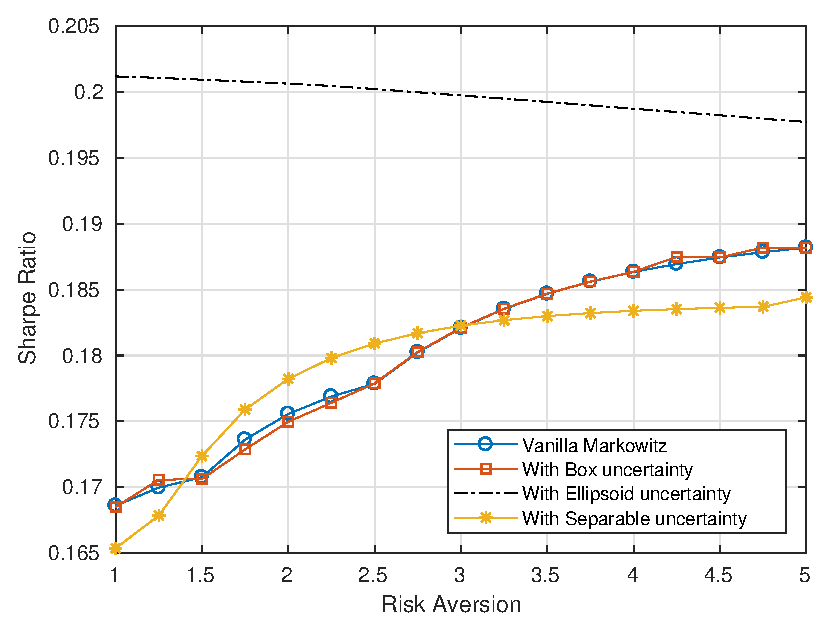
\includegraphics[height=6.7cm,width=0.52\textwidth]{bse30_simulated/sr_ideal_range_1000_sim.eps}}\\
   \caption{Efficient Frontier plot and Sharpe ratio plot for different portfolio optimization models in case of Simulated Data with 1000 samples (31 assets)}
   \label{fig:1}
\end{figure}

\begin{table}[!h]
    \centering
    \captionsetup{justification=centering}
   %\begin{tabular}{|c|c|c|c|c|c|c|c|c|c|c|c|c|}
   \begin{tabular}{||c|c|c|c|c||}
   \hline
  
%   $\lambda$ & $\sigma_{Mark}$ & $\mu_{Box}$ & $\sigma_{Box}$ & $\mu_{Ellip}$ & $\sigma_{Ellip}$ & $\mu_{Sep}$ & $\sigma_{Sep}$ & $S_{Mark}$ & $S_{Box}$ & $S_{Ellip}$ & $S_{Sep}$ \\
  
  $\lambda$ & $SR_{Mark}$ & $SR_{Box}$ & $SR_{Ellip}$ & $SR_{Sep}$ \\
  
  \hline
  2 & 0.176 & 0.175 & 0.201 & 0.178 \\
  2.5 & 0.178 & 0.178 & 0.2 & 0.181 \\
  3 & 0.182 & 0.182 & 0.2 & 0.182 \\
  3.5 & 0.185 & 0.185 & 0.199 & 0.183 \\
  4 & 0.186 & 0.186 & 0.199 & 0.183 \\
  \hline
  Avg & 0.181 & 0.181 & 0.2 & 0.182 \\
  \hline

\end{tabular}
    \caption{Comparison of different portfolio optimization models in case of Simulated Data with 1000 samples (31 assets)}
    \label{tab:1}
\end{table}

On performing the simulation study with same number of samples as in case of market data (Figure \ref{fig:2} and Table \ref{tab:2}), we observe similar results on comparing Box model with the Mark model. However, we observe slight inconsistency in performance of the Box model as evident from the plot of the Sharpe Ratio in Figure \ref{fig:2}. The efficient frontiers for the Sep and Ellip model lie below that for the Mark model. We also infer that the Sep model and the Ellip model outperform the Mark model in terms of Sharpe Ratio in the ideal range of risk-aversion. However, it is difficult to compare the performance of the Sep model with that of the Ellip model in this case since the average Sharpe Ratio for both of them is almost the same.

\begin{figure}[!h]
    %\centering
    %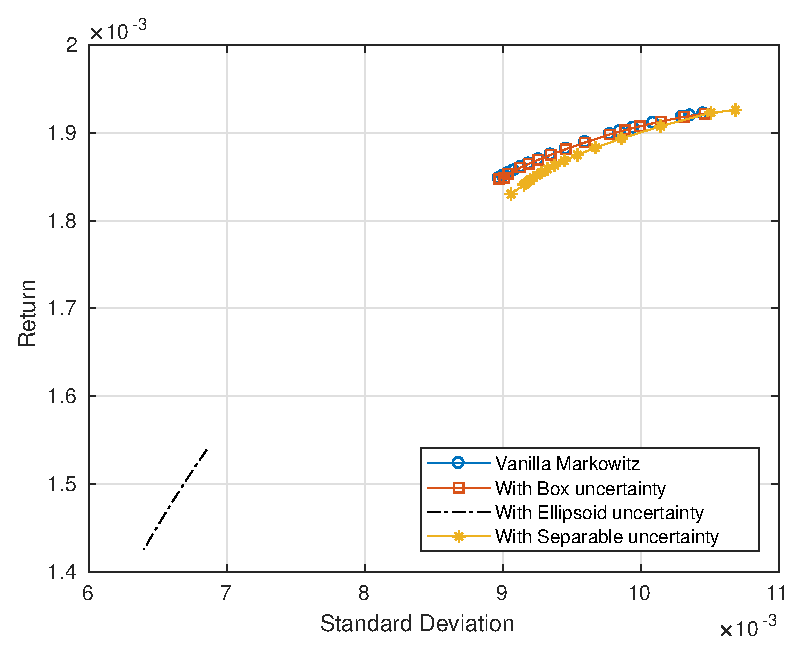
\includegraphics{bse30_simulated/ef_ideal_range_1000_sim.eps}
    %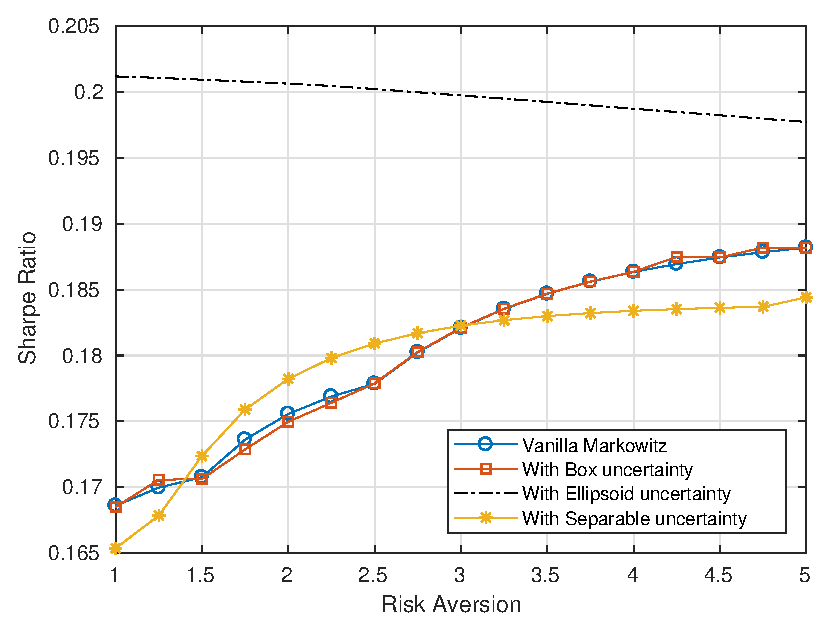
\includegraphics{bse30_simulated/sr_ideal_range_1000_sim.eps}
    
    
    \subfloat{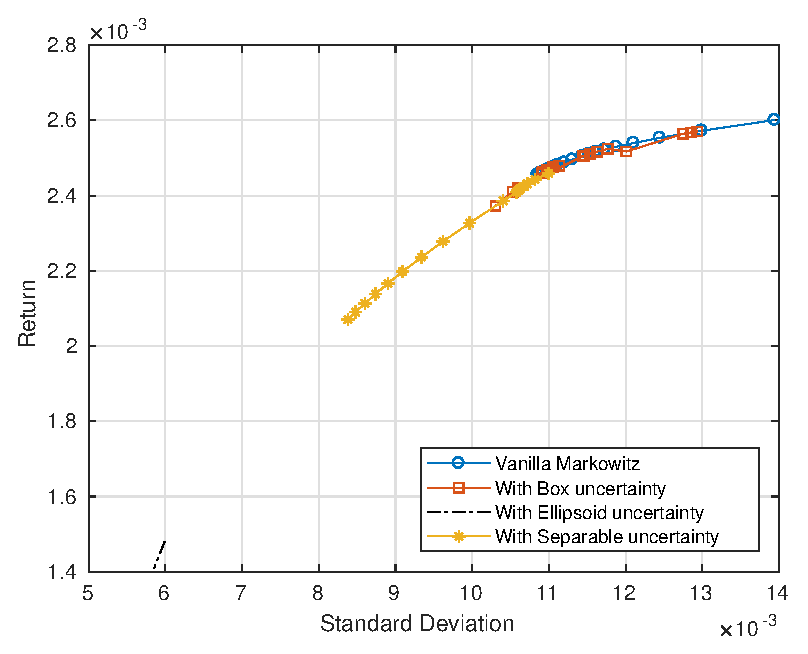
\includegraphics[height=6.9cm,width=0.5\textwidth]{bse30_simulated/ef_ideal_range_exact_sim.eps}} \hfill
   \subfloat{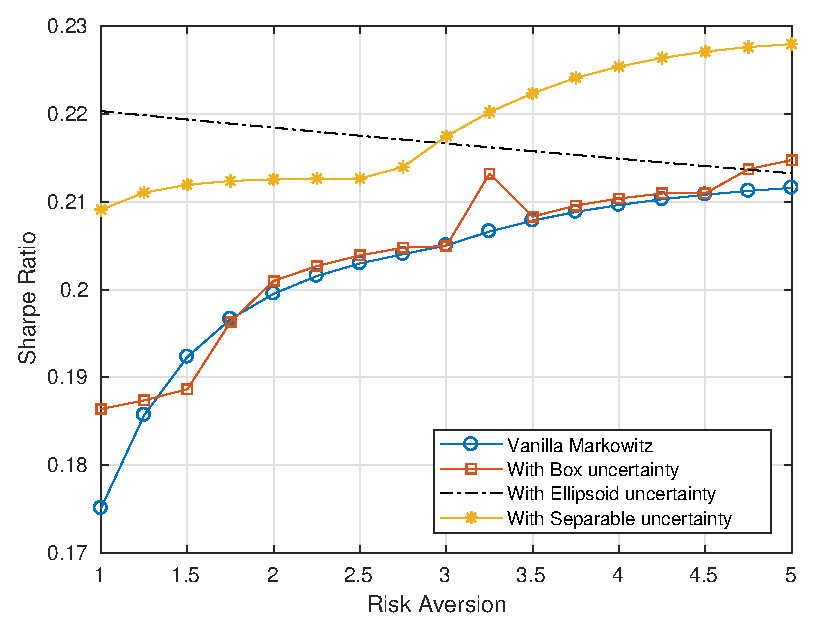
\includegraphics[height=6.7cm,width=0.52\textwidth]{bse30_simulated/sr_ideal_range_exact_sim.eps}}\\
   \caption{Efficient Frontier plot and Sharpe ratio plot for different portfolio optimization models in case of Simulated Data with same number of samples as market data (31 assets)}
   \label{fig:2}
\end{figure}

\begin{table}[!h]
    \centering
    \captionsetup{justification=centering}
   %\begin{tabular}{|c|c|c|c|c|c|c|c|c|c|c|c|c|}
   \begin{tabular}{||c|c|c|c|c||}
   \hline
  
%   $\lambda$ & $\sigma_{Mark}$ & $\mu_{Box}$ & $\sigma_{Box}$ & $\mu_{Ellip}$ & $\sigma_{Ellip}$ & $\mu_{Sep}$ & $\sigma_{Sep}$ & $S_{Mark}$ & $S_{Box}$ & $S_{Ellip}$ & $S_{Sep}$ \\
  
  $\lambda$ & $SR_{Mark}$ & $SR_{Box}$ & $SR_{Ellip}$ & $SR_{Sep}$ \\
  
  \hline
 2 & 0.2 & 0.198 & 0.218 & 0.213 \\
 2.5 & 0.203 & 0.204 & 0.218 & 0.213 \\
 3 & 0.205 & 0.207 & 0.217 & 0.217 \\
 3.5 & 0.208 & 0.209 & 0.216 & 0.222 \\
 4 & 0.21 & 0.21 & 0.215 & 0.225 \\
  \hline
  Avg & 0.205 & 0.206 & 0.217 & 0.218 \\
  \hline

\end{tabular}
    \caption{Comparison of different portfolio optimization models in case of Simulated Data with same number of samples as market data (31 assets)}
    \label{tab:2}
\end{table}

In a \say{real} market setup involving stocks comprising S\&P BSE 30, we observe that efficient frontier for the Box model almost overlaps with that for the Mark model. However, the performance of the Box model in terms of Sharpe ratio is quite inconsistent as evident from the plot in Figure \ref{fig:3}. Efficient frontier for the Sep model lies below that of the Mark model and the gap between the plots widens to a great extent, incase of the Ellip model. We also observe that the Sep model outperforms the Mark model in the ideal range of risk-aversion on taking the Sharpe Ratio into consideration as the performance measure. This is not true in case of the Ellip Model as evident from the Sharpe ratio plot in Figure \ref{fig:3}. Even from Table \ref{tab:3}, we observe that average Sharpe ratio for Ellip model is only slightly greater than that for the Mark model. Thus, unlike the simulated data, the Sep model performs superior in comparison to the Ellip model when applied to market data.
\begin{figure}[!h]
    %\centering
    %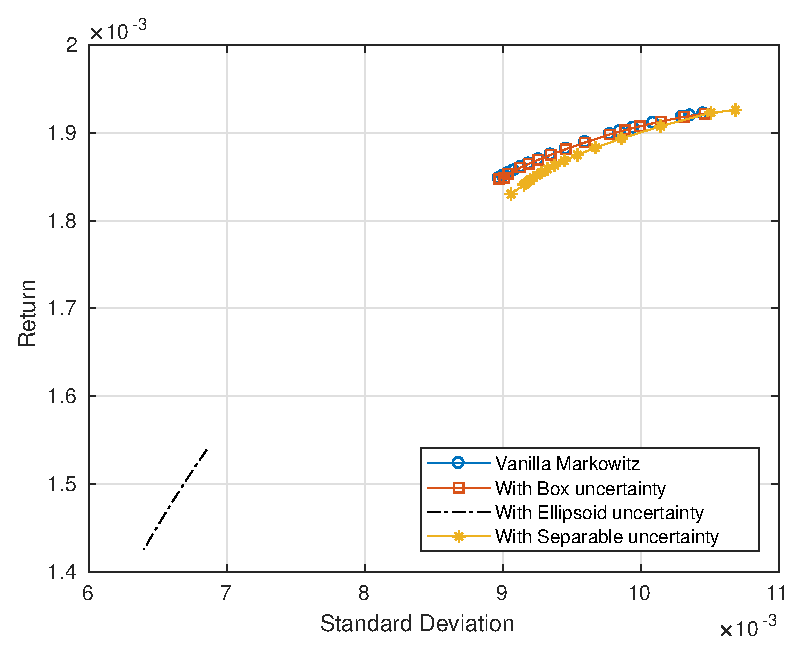
\includegraphics{bse30_simulated/ef_ideal_range_1000_sim.eps}
    %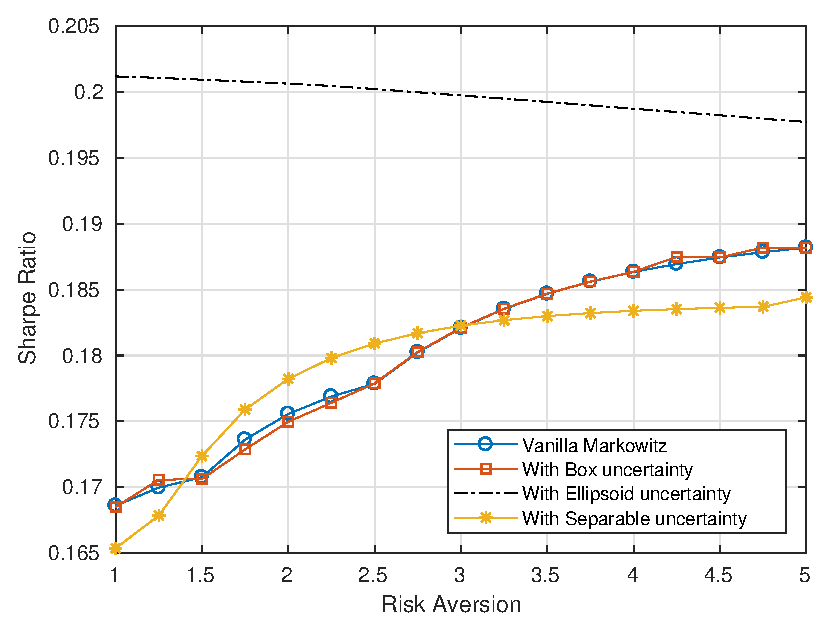
\includegraphics{bse30_simulated/sr_ideal_range_1000_sim.eps}
    
    
    \subfloat{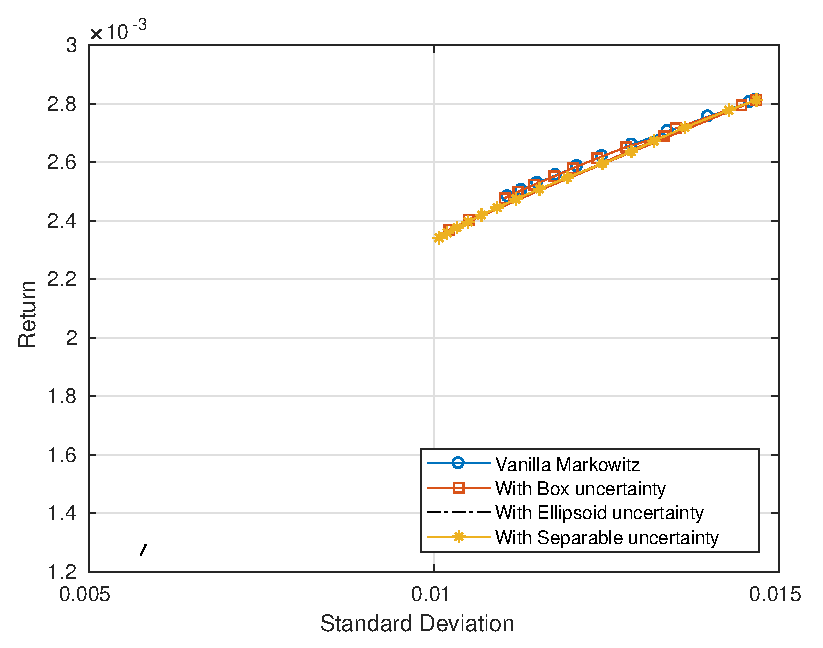
\includegraphics[height=6.9cm,width=0.5\textwidth]{bse30_market/ef_ideal_range.eps}} \hfill
   \subfloat{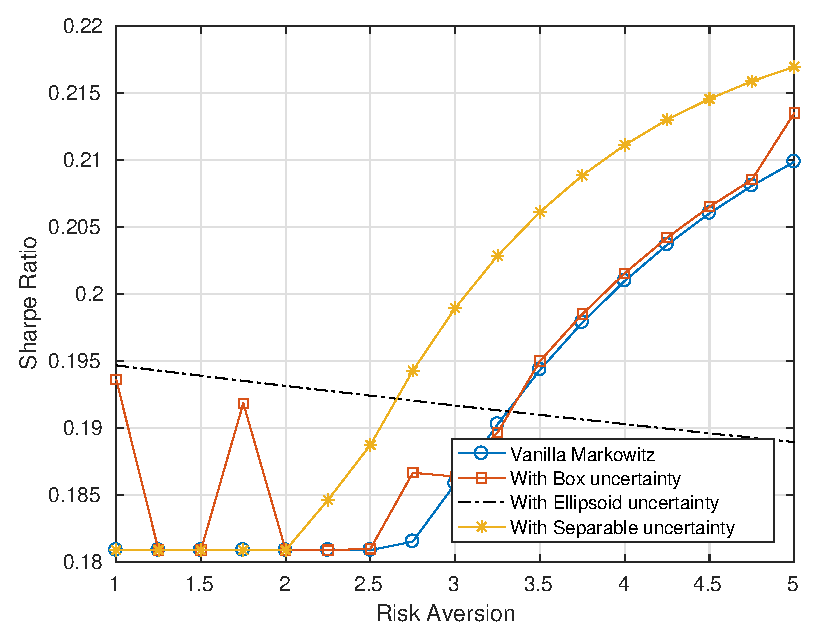
\includegraphics[height=6.7cm,width=0.52\textwidth]{bse30_market/sr_ideal_range.eps}}\\
   \caption{Efficient Frontier plot and Sharpe ratio plot for different portfolio optimization models in case of Market Data (31 assets)}
   \label{fig:3}
\end{figure}

\begin{table}[!h]
    \centering
    \captionsetup{justification=centering}
   %\begin{tabular}{|c|c|c|c|c|c|c|c|c|c|c|c|c|}
   \begin{tabular}{||c|c|c|c|c||}
   \hline
  
%   $\lambda$ & $\sigma_{Mark}$ & $\mu_{Box}$ & $\sigma_{Box}$ & $\mu_{Ellip}$ & $\sigma_{Ellip}$ & $\mu_{Sep}$ & $\sigma_{Sep}$ & $S_{Mark}$ & $S_{Box}$ & $S_{Ellip}$ & $S_{Sep}$ \\
  
  $\lambda$ & $SR_{Mark}$ & $SR_{Box}$ & $SR_{Ellip}$ & $SR_{Sep}$ \\
  
  \hline
 2 & 0.181 & 0.181 & 0.193 & 0.186 \\
 2.5 & 0.181 & 0.181 & 0.192 & 0.193 \\
 3 & 0.186 & 0.191 & 0.192 & 0.202 \\
 3.5 & 0.194 & 0.195 & 0.191 & 0.209 \\
 4 & 0.201 & 0.202 & 0.19 & 0.213 \\
  \hline
  Avg & 0.189 & 0.19 & 0.192 & 0.2 \\
  \hline

\end{tabular}
    \caption{Comparison of different portfolio optimization models in case of Market Data (31 assets)}
    \label{tab:3}
\end{table}

A common observation that could be inferred from three cases considered in the scenario involving less number of assets ($N=31$) is that the Sep and Ellip models perform superior or equivalent in comparison to the Mark model in the ideal range of risk-aversion.


\section{Performance with $N=98$ Assets}

We now analyze the scenario involving $N=98$ assets. On applying robust models along with the Mark model on a simulated data having 1000 samples, we observe results similar to the corresponding case for the previous scenario when we compared the Box model with the Mark model. This is evident from the coinciding plots of the efficient frontier and the Sharpe ratio for both the models in Figure \ref{fig:4}. Contrary to the similar case for the scenario involving less number of assets ($N=31$), we observe that not only does the Ellip model but also the Sep model outperforms the Mark model taking into consideration the portfolios constructed in the ideal range of risk-aversion. Additionally, from Table \ref{tab:4}, we infer that the Ellip model performs superior in comparison to the Sep model in terms of greater average value of the Sharpe ratio.
\begin{figure}[!h]
    %\centering
    %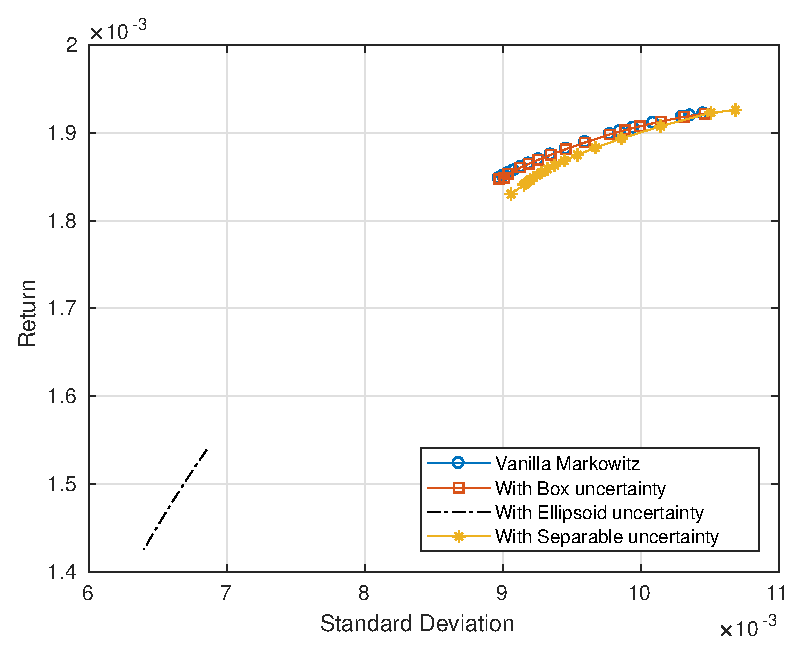
\includegraphics{bse30_simulated/ef_ideal_range_1000_sim.eps}
    %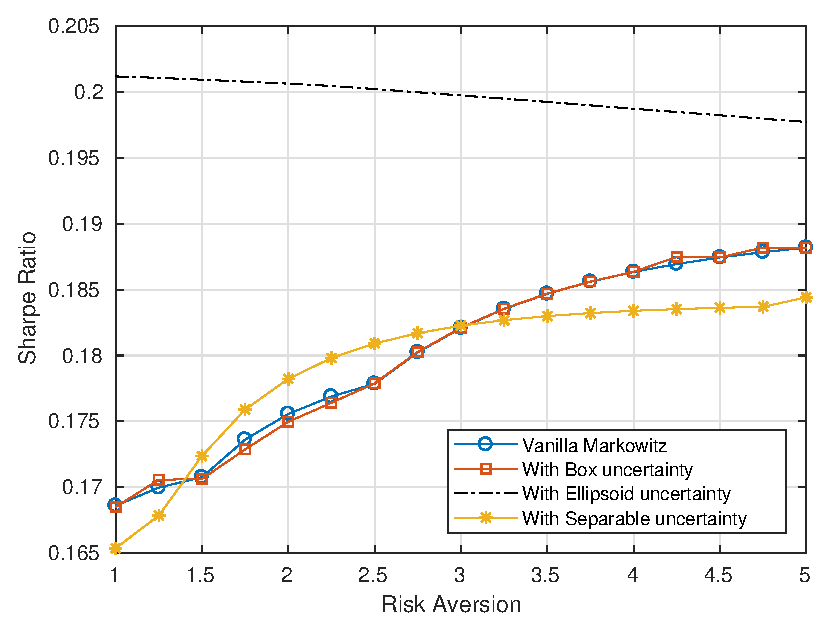
\includegraphics{bse30_simulated/sr_ideal_range_1000_sim.eps}
    
    
    \subfloat{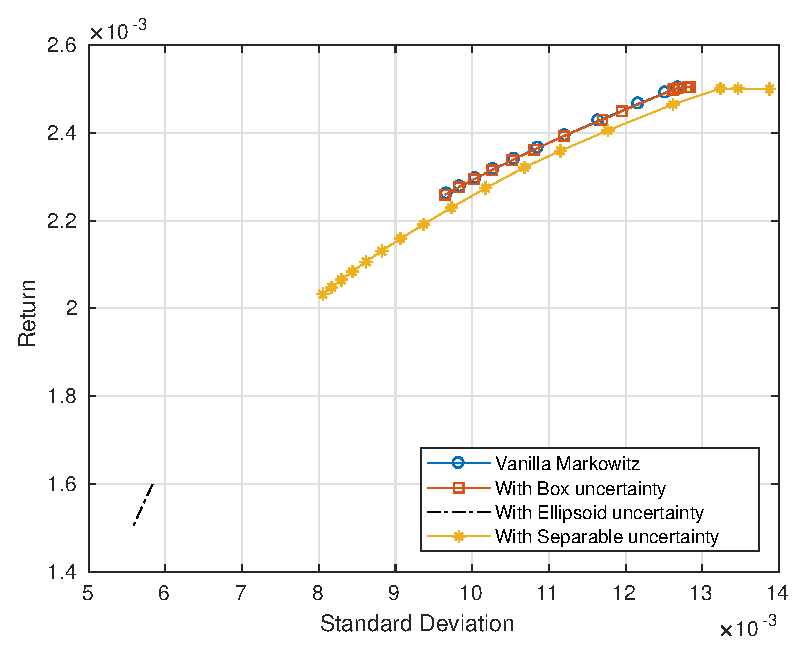
\includegraphics[height=6.9cm,width=0.5\textwidth]{bse100_simulated/ef_ideal_range_1000_sim.eps}} \hfill
   \subfloat{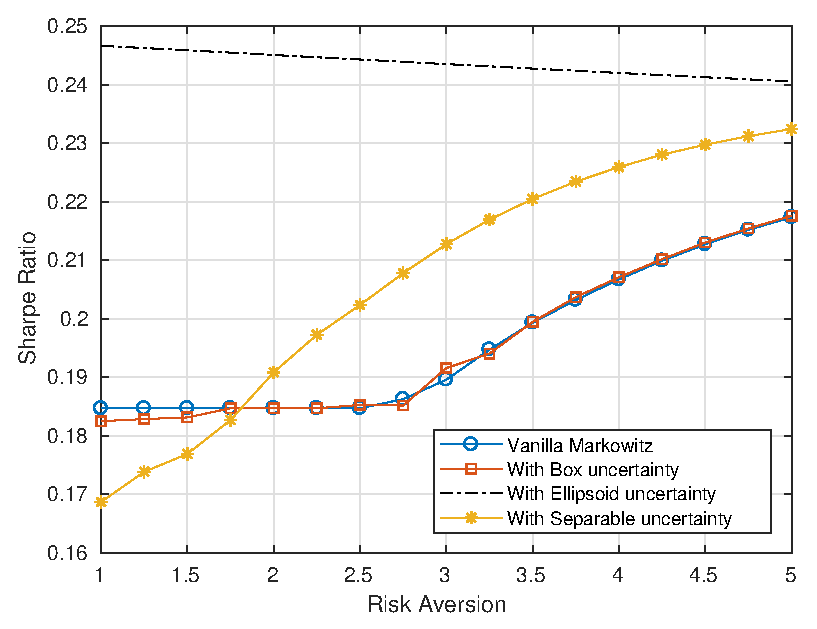
\includegraphics[height=6.7cm,width=0.52\textwidth]{bse100_simulated/sr_ideal_range_1000_sim.eps}}\\
   \caption{Efficient Frontier plot and Sharpe ratio plot for different portfolio optimization models in case of Simulated Data with 1000 samples (98 assets)}
   \label{fig:4}
\end{figure}

\begin{table}[!h]
    \centering
    \captionsetup{justification=centering}
   %\begin{tabular}{|c|c|c|c|c|c|c|c|c|c|c|c|c|}
   \begin{tabular}{||c|c|c|c|c||}
   \hline
  
%   $\lambda$ & $\sigma_{Mark}$ & $\mu_{Box}$ & $\sigma_{Box}$ & $\mu_{Ellip}$ & $\sigma_{Ellip}$ & $\mu_{Sep}$ & $\sigma_{Sep}$ & $S_{Mark}$ & $S_{Box}$ & $S_{Ellip}$ & $S_{Sep}$ \\
  
  $\lambda$ & $SR_{Mark}$ & $SR_{Box}$ & $SR_{Ellip}$ & $SR_{Sep}$ \\
  
  \hline
 2 & 0.185 & 0.185 & 0.245 & 0.191 \\
 2.5 & 0.185 & 0.185 & 0.244 & 0.202 \\
 3 & 0.19 & 0.192 & 0.244 & 0.213 \\
 3.5 & 0.199 & 0.199 & 0.243 & 0.221 \\
 4 & 0.207 & 0.207 & 0.242 & 0.226 \\
  \hline
  Avg & 0.193 & 0.194 & 0.244 & 0.21 \\
  \hline

\end{tabular}
    \caption{Comparison of different portfolio optimization models in case of Simulated Data with 1000 samples (98 assets)}
    \label{tab:4}
\end{table}

Figure \ref{fig:5} and Table \ref{tab:5} present the results of simulation study with same number of samples as that of log-returns of S\&P BSE 100 data. Results observed on comparing the Box model with the Mark model are similar to the previous case of $1000$ simulated samples.  In the ideal range of risk aversion, we observe that efficient frontier for the Ellip as well as the Sep model lie below the Mark model. Additionally, both the models perform better than the Mark model in terms of the Sharpe Ratio. From the Sharpe Ratio plot in Figure \ref{fig:5}, it is difficult to compare the Sep model and the Ellip model since each outperforms the other in a different sub-interval of risk-aversion. The similar values of the average Sharpe ratio in Table \ref{tab:5} supports the claim of equivalent performance of these two models in this case.

\begin{figure}[!h]
    %\centering
    %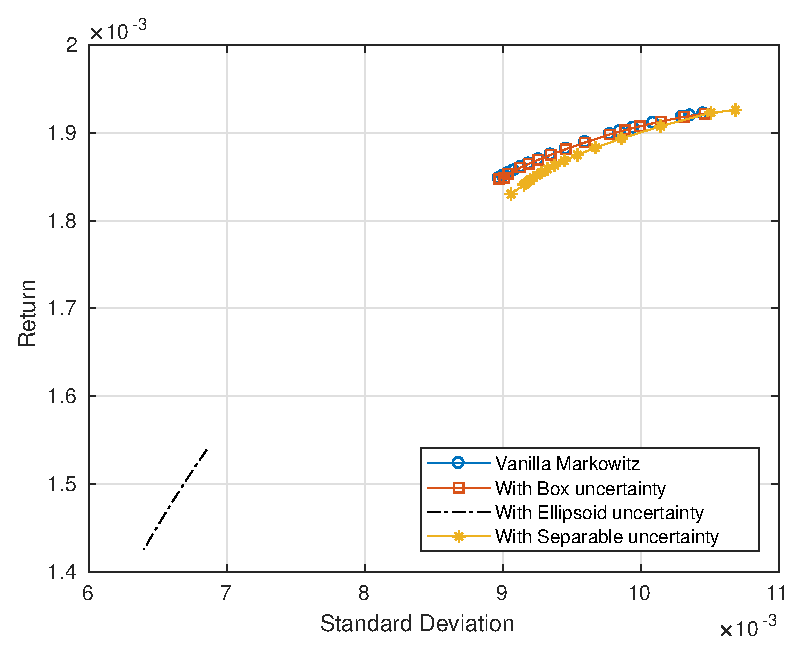
\includegraphics{bse30_simulated/ef_ideal_range_1000_sim.eps}
    %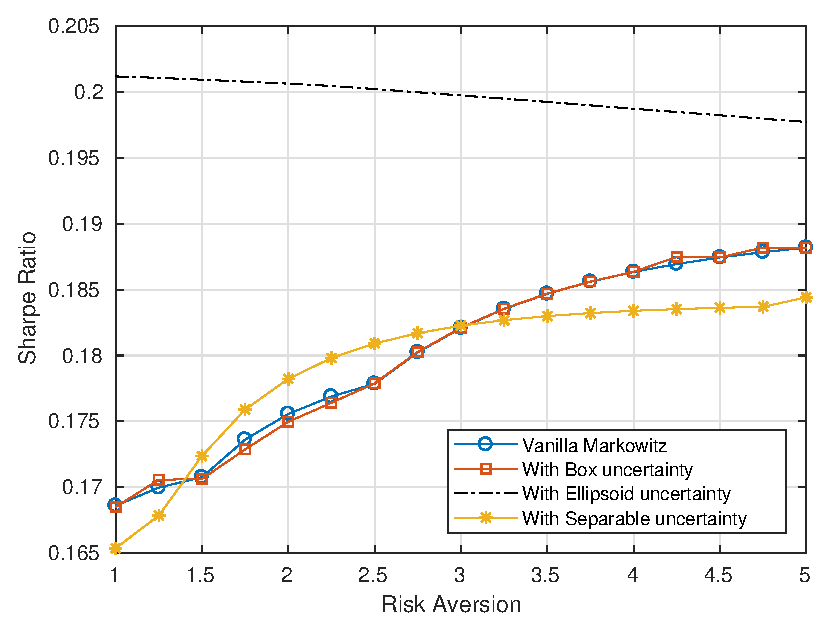
\includegraphics{bse30_simulated/sr_ideal_range_1000_sim.eps}
    
    
    \subfloat{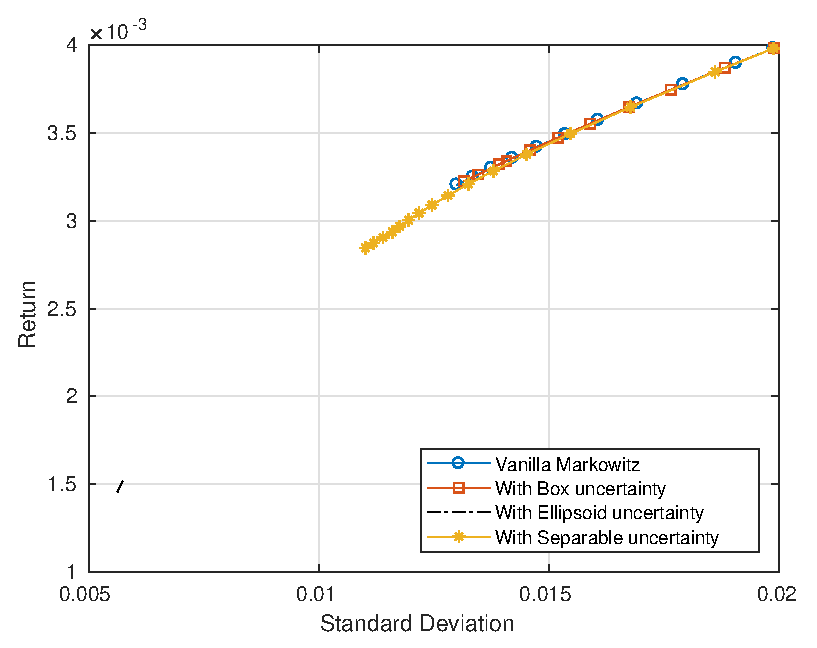
\includegraphics[height=6.9cm,width=0.5\textwidth]{bse100_simulated/ef_ideal_range_exact_sim.eps}} \hfill
   \subfloat{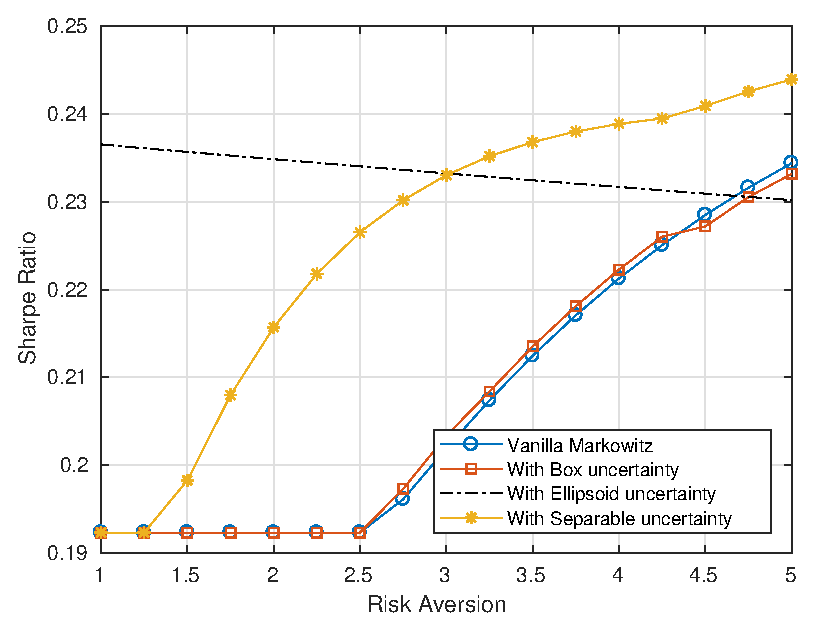
\includegraphics[height=6.7cm,width=0.52\textwidth]{bse100_simulated/sr_ideal_range_exact_sim.eps}}\\
   \caption{Efficient Frontier plot and Sharpe ratio plot for different portfolio optimization models in case of Simulated Data with same number of samples as market data (98 assets)}
   \label{fig:5}
\end{figure}

\begin{table}[!h]
    \centering
    \captionsetup{justification=centering}
   %\begin{tabular}{|c|c|c|c|c|c|c|c|c|c|c|c|c|}
   \begin{tabular}{||c|c|c|c|c||}
   \hline
  
%   $\lambda$ & $\sigma_{Mark}$ & $\mu_{Box}$ & $\sigma_{Box}$ & $\mu_{Ellip}$ & $\sigma_{Ellip}$ & $\mu_{Sep}$ & $\sigma_{Sep}$ & $S_{Mark}$ & $S_{Box}$ & $S_{Ellip}$ & $S_{Sep}$ \\
  
  $\lambda$ & $SR_{Mark}$ & $SR_{Box}$ & $SR_{Ellip}$ & $SR_{Sep}$ \\
  
  \hline
 2 & 0.192 & 0.192 & 0.235 & 0.216 \\
 2.5 & 0.192 & 0.192 & 0.234 & 0.227 \\
 3 & 0.202 & 0.203 & 0.233 & 0.233 \\
 3.5 & 0.212 & 0.213 & 0.232 & 0.237 \\
 4 & 0.221 & 0.222 & 0.232 & 0.239 \\
  \hline
  Avg & 0.204 & 0.205 & 0.233 & 0.23 \\
  \hline

\end{tabular}
    \caption{Comparison of different portfolio optimization models in case of Simulated Data with same number of samples as market data (98 assets)}
    \label{tab:5}
\end{table}

The results for the case involving the market data (that contains log-returns of stocks comprising BSE 100) are  presented in Figure \ref{fig:6} and Table \ref{tab:6}. The efficient frontier plot leads to observations similar to the previous case. However, there is a slight inconsistency in the performance of the Box model as observed from the plot of the Sharpe Ratio in Figure \ref{fig:6}. The robust portfolios constructed using the Sep and the Ellip model outperform the ones constructed using the Mark model in the ideal range of risk-aversion. Additionally, the Ellip model performs slightly better than the Sep model as evident from the Sharpe Ratio plot. Marginal difference in average Sharpe ratio between these two models supports this inference.
\begin{figure}[!h]
    %\centering
    %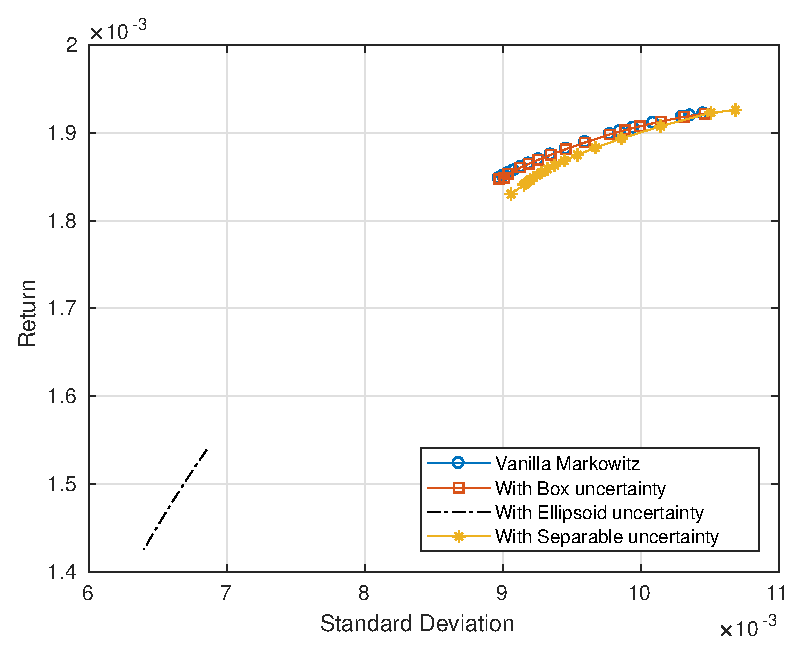
\includegraphics{bse30_simulated/ef_ideal_range_1000_sim.eps}
    %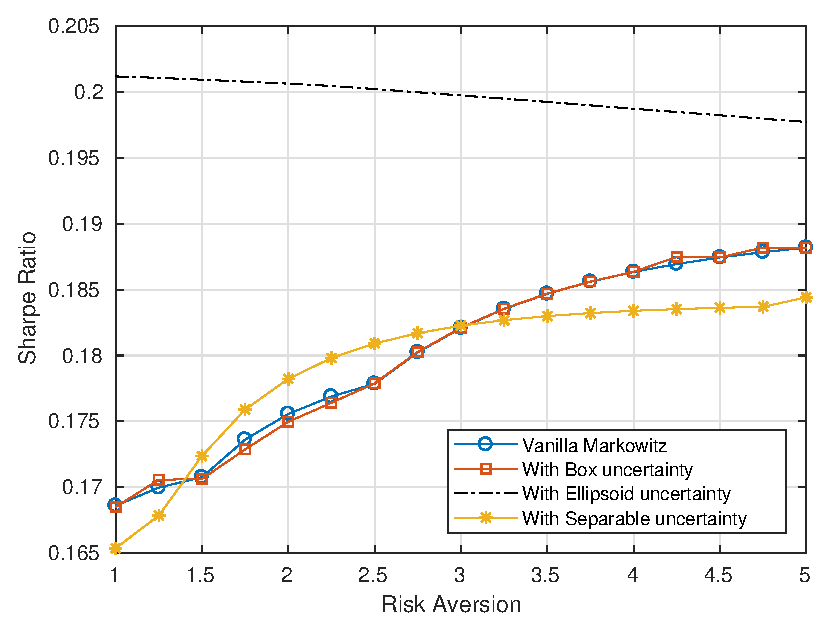
\includegraphics{bse30_simulated/sr_ideal_range_1000_sim.eps}
    
    
    \subfloat{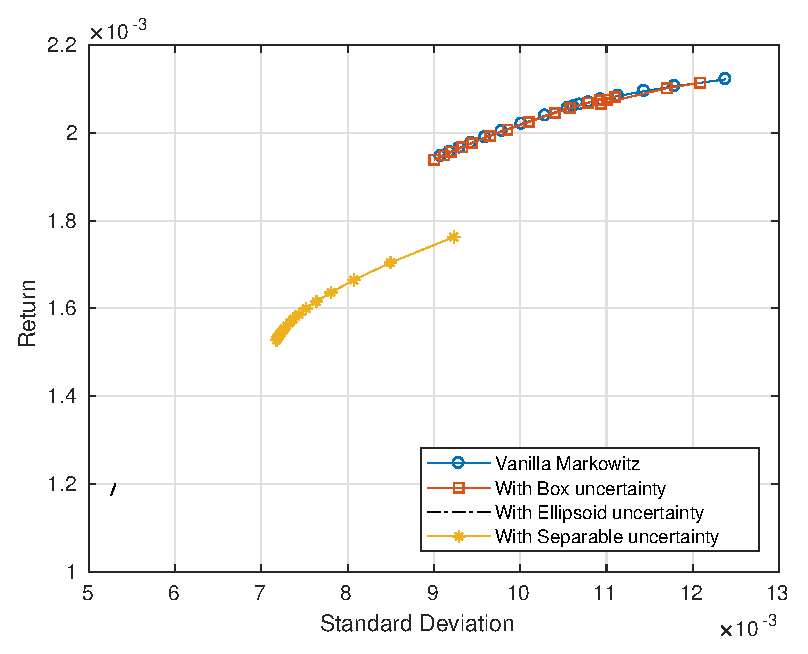
\includegraphics[height=6.9cm,width=0.5\textwidth]{bse100_market/ef_ideal_range.eps}} \hfill
   \subfloat{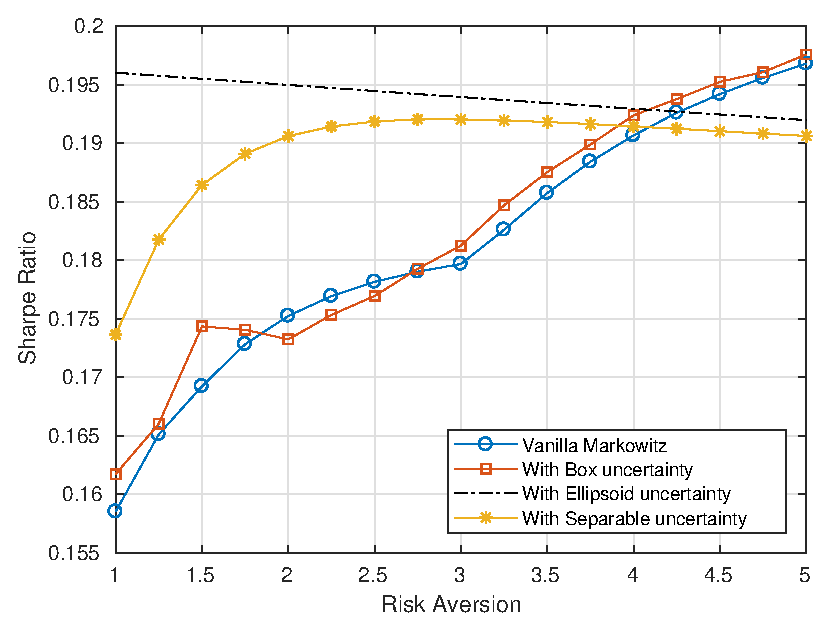
\includegraphics[height=6.7cm,width=0.52\textwidth]{bse100_market/sr_ideal_range.eps}}\\
   \caption{Efficient Frontier plot and Sharpe ratio plot for different portfolio optimization models in case of Market Data (98 assets)}
   \label{fig:6}
\end{figure}

\begin{table}[!h]
    \centering
    \captionsetup{justification=centering}
   %\begin{tabular}{|c|c|c|c|c|c|c|c|c|c|c|c|c|}
   \begin{tabular}{||c|c|c|c|c||}
   \hline
  
%   $\lambda$ & $\sigma_{Mark}$ & $\mu_{Box}$ & $\sigma_{Box}$ & $\mu_{Ellip}$ & $\sigma_{Ellip}$ & $\mu_{Sep}$ & $\sigma_{Sep}$ & $S_{Mark}$ & $S_{Box}$ & $S_{Ellip}$ & $S_{Sep}$ \\
  
  $\lambda$ & $SR_{Mark}$ & $SR_{Box}$ & $SR_{Ellip}$ & $SR_{Sep}$ \\
  
  \hline
2 & 0.175 & 0.173 & 0.195 & 0.193 \\
2.5 & 0.178 & 0.177 & 0.194 & 0.193 \\
3 & 0.18 & 0.181 & 0.194 & 0.193 \\
3.5 & 0.186 & 0.188 & 0.193 & 0.192 \\
4 & 0.191 & 0.192 & 0.193 & 0.192 \\
  \hline
  Avg & 0.182 & 0.182 & 0.194 & 0.192 \\
  \hline

\end{tabular}
    \caption{Comparison of different portfolio optimization models in case of Market Data (98 assets)}
    \label{tab:6}
\end{table} 

We draw a common inference from the three cases considered in the scenario involving greater number of assets, \textit{i.e.}, Sep and Ellip model outperform the Markowitz model in the ideal range of risk aversion.







